\documentclass[11pt,a4paper]{article}

\usepackage[margin=2.3cm]{geometry}
\usepackage[T1]{fontenc}
\usepackage{lmodern}
\usepackage{microtype}
\usepackage{amsmath}
\usepackage{booktabs}
\usepackage{tabularx}
\usepackage{graphicx}
\usepackage{xcolor}
\usepackage{enumitem}
\usepackage{needspace}
\usepackage{tikz}
\usetikzlibrary{positioning,arrows.meta,shapes.geometric,calc}
\usepackage[hidelinks]{hyperref}

\setlist{itemsep=2pt,topsep=4pt}
\graphicspath{{figures/}}
% Generated by report/make_final_figures.py; do not edit by hand.
\newcommand{\fN}{22}
\newcommand{\fInterviews}{110}
\newcommand{\fPlanted}{32}
\newcommand{\fAccBOne}{52\%}
\newcommand{\fAccLowBOne}{39\%}
\newcommand{\fAccHighBOne}{64\%}
\newcommand{\fMaeBOne}{0.52}
\newcommand{\fExchBOne}{12.0}
\newcommand{\fMainBOne}{12.0}
\newcommand{\fFollowBOne}{0.0}
\newcommand{\fPrematureBOne}{0\%}
\newcommand{\fCoverageBOne}{90\%}
\newcommand{\fReviewBOne}{55\%}
\newcommand{\fRightBOne}{9}
\newcommand{\fWrongBOne}{1}
\newcommand{\fReviewNBOne}{12}
\newcommand{\fCallsBOne}{37}
\newcommand{\fGradingMatchBOne}{88\%}
\newcommand{\fAccAdapt}{62\%}
\newcommand{\fAccLowAdapt}{50\%}
\newcommand{\fAccHighAdapt}{74\%}
\newcommand{\fMaeAdapt}{0.39}
\newcommand{\fExchAdapt}{12.0}
\newcommand{\fMainAdapt}{12.0}
\newcommand{\fFollowAdapt}{0.0}
\newcommand{\fPrematureAdapt}{0\%}
\newcommand{\fCoverageAdapt}{76\%}
\newcommand{\fReviewAdapt}{55\%}
\newcommand{\fRightAdapt}{10}
\newcommand{\fWrongAdapt}{0}
\newcommand{\fReviewNAdapt}{12}
\newcommand{\fCallsAdapt}{37}
\newcommand{\fGradingMatchAdapt}{85\%}
\newcommand{\fAccFull}{53\%}
\newcommand{\fAccLowFull}{41\%}
\newcommand{\fAccHighFull}{65\%}
\newcommand{\fMaeFull}{0.48}
\newcommand{\fExchFull}{20.1}
\newcommand{\fMainFull}{13.8}
\newcommand{\fFollowFull}{6.3}
\newcommand{\fPrematureFull}{77\%}
\newcommand{\fCoverageFull}{74\%}
\newcommand{\fReviewFull}{59\%}
\newcommand{\fRightFull}{9}
\newcommand{\fWrongFull}{0}
\newcommand{\fReviewNFull}{13}
\newcommand{\fCallsFull}{113}
\newcommand{\fGradingMatchFull}{87\%}
\newcommand{\fAccBlind}{62\%}
\newcommand{\fAccLowBlind}{50\%}
\newcommand{\fAccHighBlind}{73\%}
\newcommand{\fMaeBlind}{0.38}
\newcommand{\fExchBlind}{21.3}
\newcommand{\fMainBlind}{14.0}
\newcommand{\fFollowBlind}{7.2}
\newcommand{\fPrematureBlind}{68\%}
\newcommand{\fCoverageBlind}{62\%}
\newcommand{\fReviewBlind}{50\%}
\newcommand{\fRightBlind}{11}
\newcommand{\fWrongBlind}{0}
\newcommand{\fReviewNBlind}{11}
\newcommand{\fCallsBlind}{120}
\newcommand{\fGradingMatchBlind}{85\%}
\newcommand{\fAccAfour}{70\%}
\newcommand{\fAccLowAfour}{61\%}
\newcommand{\fAccHighAfour}{79\%}
\newcommand{\fMaeAfour}{0.30}
\newcommand{\fExchAfour}{18.9}
\newcommand{\fMainAfour}{14.0}
\newcommand{\fFollowAfour}{4.9}
\newcommand{\fPrematureAfour}{50\%}
\newcommand{\fCoverageAfour}{85\%}
\newcommand{\fReviewAfour}{36\%}
\newcommand{\fRightAfour}{14}
\newcommand{\fWrongAfour}{0}
\newcommand{\fReviewNAfour}{8}
\newcommand{\fCallsAfour}{65}
\newcommand{\fGradingMatchAfour}{90\%}
\newcommand{\fOverBOne}{24}
\newcommand{\fUnderBOne}{8}
\newcommand{\fConfStopsBOne}{0}
\newcommand{\fConfWrongBOne}{0}
\newcommand{\fConfSkillsBOne}{0}
\newcommand{\fConfWrongPyBOne}{0}
\newcommand{\fConfWrongSqlBOne}{0}
\newcommand{\fConfWrongDsBOne}{0}
\newcommand{\fZeroWrongBOne}{0}
\newcommand{\fZeroBOne}{0}
\newcommand{\fConfTwoOffBOne}{0}
\newcommand{\fHeldBeliefBOne}{0.5}
\newcommand{\fOverAdapt}{20}
\newcommand{\fUnderAdapt}{5}
\newcommand{\fConfStopsAdapt}{0}
\newcommand{\fConfWrongAdapt}{0}
\newcommand{\fConfSkillsAdapt}{0}
\newcommand{\fConfWrongPyAdapt}{0}
\newcommand{\fConfWrongSqlAdapt}{0}
\newcommand{\fConfWrongDsAdapt}{0}
\newcommand{\fZeroWrongAdapt}{0}
\newcommand{\fZeroAdapt}{0}
\newcommand{\fConfTwoOffAdapt}{0}
\newcommand{\fHeldBeliefAdapt}{1.1}
\newcommand{\fOverFull}{17}
\newcommand{\fUnderFull}{14}
\newcommand{\fConfStopsFull}{20}
\newcommand{\fConfWrongFull}{29}
\newcommand{\fConfSkillsFull}{60}
\newcommand{\fConfWrongPyFull}{13}
\newcommand{\fConfWrongSqlFull}{6}
\newcommand{\fConfWrongDsFull}{10}
\newcommand{\fZeroWrongFull}{2}
\newcommand{\fZeroFull}{5}
\newcommand{\fConfTwoOffFull}{1}
\newcommand{\fHeldBeliefFull}{1.5}
\newcommand{\fOverBlind}{17}
\newcommand{\fUnderBlind}{8}
\newcommand{\fConfStopsBlind}{18}
\newcommand{\fConfWrongBlind}{23}
\newcommand{\fConfSkillsBlind}{54}
\newcommand{\fConfWrongPyBlind}{9}
\newcommand{\fConfWrongSqlBlind}{6}
\newcommand{\fConfWrongDsBlind}{8}
\newcommand{\fZeroWrongBlind}{3}
\newcommand{\fZeroBlind}{4}
\newcommand{\fConfTwoOffBlind}{0}
\newcommand{\fHeldBeliefBlind}{1.3}
\newcommand{\fOverAfour}{16}
\newcommand{\fUnderAfour}{4}
\newcommand{\fConfStopsAfour}{15}
\newcommand{\fConfWrongAfour}{15}
\newcommand{\fConfSkillsAfour}{45}
\newcommand{\fConfWrongPyAfour}{7}
\newcommand{\fConfWrongSqlAfour}{2}
\newcommand{\fConfWrongDsAfour}{6}
\newcommand{\fZeroWrongAfour}{2}
\newcommand{\fZeroAfour}{4}
\newcommand{\fConfTwoOffAfour}{0}
\newcommand{\fHeldBeliefAfour}{0.8}
\newcommand{\fRecallFull}{34\%}
\newcommand{\fPrecisionFull}{58\%}
\newcommand{\fRecallLowFull}{19\%}
\newcommand{\fRecallHighFull}{50\%}
\newcommand{\fPrecisionLowFull}{35\%}
\newcommand{\fPrecisionHighFull}{82\%}
\newcommand{\fFoundFull}{11}
\newcommand{\fConfirmedFull}{19}
\newcommand{\fSuspectedFull}{59}
\newcommand{\fDisputedFull}{2}
\newcommand{\fFalseAlarmFull}{0.0\%}
\newcommand{\fRecallBlind}{38\%}
\newcommand{\fPrecisionBlind}{57\%}
\newcommand{\fRecallLowBlind}{20\%}
\newcommand{\fRecallHighBlind}{54\%}
\newcommand{\fPrecisionLowBlind}{39\%}
\newcommand{\fPrecisionHighBlind}{76\%}
\newcommand{\fFoundBlind}{12}
\newcommand{\fConfirmedBlind}{21}
\newcommand{\fSuspectedBlind}{64}
\newcommand{\fDisputedBlind}{6}
\newcommand{\fFalseAlarmBlind}{0.7\%}
\newcommand{\fRecallAfour}{56\%}
\newcommand{\fPrecisionAfour}{20\%}
\newcommand{\fRecallLowAfour}{37\%}
\newcommand{\fRecallHighAfour}{73\%}
\newcommand{\fPrecisionLowAfour}{13\%}
\newcommand{\fPrecisionHighAfour}{26\%}
\newcommand{\fFoundAfour}{18}
\newcommand{\fConfirmedAfour}{92}
\newcommand{\fSuspectedAfour}{0}
\newcommand{\fDisputedAfour}{0}
\newcommand{\fFalseAlarmAfour}{0.0\%}
\newcommand{\fFullVsFixedSkillAccuracyDiff}{+1.5}
\newcommand{\fFullVsFixedSkillAccuracyLow}{$-$16.7}
\newcommand{\fFullVsFixedSkillAccuracyHigh}{+19.7}
\newcommand{\fFullVsFixedMeanExchangesDiff}{+8.1}
\newcommand{\fFullVsFixedMeanExchangesLow}{+7.0}
\newcommand{\fFullVsFixedMeanExchangesHigh}{+9.4}
\newcommand{\fFullVsFixedMaeDiff}{$-$0.03}
\newcommand{\fFullVsFixedMaeLow}{$-$0.21}
\newcommand{\fFullVsFixedMaeHigh}{+0.15}
\newcommand{\fAdaptVsFixedSkillAccuracyDiff}{+10.6}
\newcommand{\fAdaptVsFixedSkillAccuracyLow}{$-$4.5}
\newcommand{\fAdaptVsFixedSkillAccuracyHigh}{+25.8}
\newcommand{\fAdaptVsFixedMaeDiff}{$-$0.12}
\newcommand{\fAdaptVsFixedMaeLow}{$-$0.27}
\newcommand{\fAdaptVsFixedMaeHigh}{+0.05}
\newcommand{\fFullVsAfourRecallDiff}{$-$21.9}
\newcommand{\fFullVsAfourRecallLow}{$-$35.5}
\newcommand{\fFullVsAfourRecallHigh}{$-$9.4}
\newcommand{\fFullVsAfourPrecisionDiff}{+38.3}
\newcommand{\fFullVsAfourPrecisionLow}{+18.7}
\newcommand{\fFullVsAfourPrecisionHigh}{+62.3}
\newcommand{\fFullVsAfourFalseAlarmRateDiff}{+0.0}
\newcommand{\fFullVsAfourFalseAlarmRateLow}{+0.0}
\newcommand{\fFullVsAfourFalseAlarmRateHigh}{+0.0}
\newcommand{\fFullVsAfourSkillAccuracyDiff}{$-$16.7}
\newcommand{\fFullVsAfourSkillAccuracyLow}{$-$28.8}
\newcommand{\fFullVsAfourSkillAccuracyHigh}{$-$4.5}
\newcommand{\fFullVsAfourMeanExchangesDiff}{+1.2}
\newcommand{\fFullVsAfourMeanExchangesLow}{+0.2}
\newcommand{\fFullVsAfourMeanExchangesHigh}{+2.4}
\newcommand{\fBlindVsFullSkillAccuracyDiff}{+9.1}
\newcommand{\fBlindVsFullSkillAccuracyLow}{$-$3.0}
\newcommand{\fBlindVsFullSkillAccuracyHigh}{+21.2}
\newcommand{\fBlindVsFullRecallDiff}{+3.1}
\newcommand{\fBlindVsFullRecallLow}{$-$15.2}
\newcommand{\fBlindVsFullRecallHigh}{+22.6}
\newcommand{\fBlindVsFullTopicCoverageDiff}{$-$11.4}
\newcommand{\fBlindVsFullTopicCoverageLow}{$-$16.7}
\newcommand{\fBlindVsFullTopicCoverageHigh}{$-$5.8}


\newcommand{\pass}{\textcolor[HTML]{0a7d0a}{\textbf{met}}}
\newcommand{\fail}{\textcolor[HTML]{b02f2f}{\textbf{not met}}}
\newcommand{\open}{\textcolor[HTML]{8a6d00}{\textbf{not settled}}}
\newcommand{\ci}[2]{{\small[#1, #2]}}

\title{An Adaptive Technical Interviewer with a\\Theory of Mind of the Candidate\\[4pt]\large Final report}
\author{Team ``Claude lag gaye'': Kushal Mukherjee (2025201072) \and Srinjoy Sengupta (2025202010)
  \and Nilkanta Karak (2025201031) \and Souradeep Das (2025201004)}
\date{November 2026\\[4pt]\small Code: \url{https://github.com/Srinjoy003/LMA-RAG}}

\begin{document}
\maketitle

\begin{abstract}
A good interviewer does not only mark answers right or wrong; it forms a view of what the candidate
\emph{believes}, and asks the next question to test that view. We built an interviewer for junior
technical screening in Python, SQL and data structures with this \textbf{theory of mind} at its
centre. For every answer it decides whether the candidate does not know, slipped, misread the
question, or holds a specific false belief; it keeps each attributed belief as a hypothesis, steers
the interview to test it on a second question, confirms it only with the candidate's own words as
evidence, and withdraws it when the candidate contradicts it. Alongside this it estimates a level per
skill, picks questions to reduce its uncertainty, stops when confident, and leaves the hiring decision
to a human. Five systems interviewed the same \fN{} simulated candidates (\fInterviews{} interviews).
\textbf{With the theory of mind, \fPrecisionFull{} of the beliefs the system attributes to a candidate
are correct, against \fPrecisionAfour{} without it} (difference \fFullVsAfourPrecisionDiff{} points,
95\% interval \fFullVsAfourPrecisionLow{} to \fFullVsAfourPrecisionHigh{}), and it never attributed a
false belief to a correct answer. It is more cautious: it confirms \fRecallFull{} of the planted
beliefs against \fRecallAfour{}. Adaptive question choice judged \fAccAdapt{} of skill levels correctly
against \fAccBOne{} for a fixed interview of the same length. Probing beliefs has a cost: the full
system was not more accurate on levels (\fAccFull{}) and asked more (\fExchFull{} exchanges against
\fExchBOne{}).
\end{abstract}

\section{Introduction}

A screening interview has to judge several skills with a handful of questions. Fixed question lists
waste questions on skills that are already clear and leave others under-tested. LLM interviewers
make screening cheap, but they decide what to ask and when to stop from a prompt alone, with no
record of how sure they are. Adaptive testing solves this for multiple-choice tests by asking the
most informative question and stopping once the estimate is precise \cite{zhuang2024}, and
TestAgent \cite{yu2025} brings the idea to conversational assessment. We apply it to open answers
across several skills.

Adaptive testing tracks \emph{how much} a candidate knows. A human interviewer also tracks \emph{what
the candidate thinks}: after a wrong answer they ask themselves whether the candidate simply does not
know, made a careless slip, misread the question, or confidently holds a wrong idea, and they choose
the next question to find out. This is a theory of mind of the candidate: attributing beliefs to
another person from what they say, holding those beliefs as hypotheses, and revising them as evidence
arrives. The distinction matters for feedback and for hiring, because a false belief (``\texttt{COUNT}
counts \texttt{NULL}s'') needs different training from a gap in knowledge. Our system makes this
theory of mind explicit (Section~\ref{sec:tom}), and the experiment tests whether it works. Our two
research questions:

\begin{description}[leftmargin=1.2cm,style=nextline]
  \item[RQ1] Can uncertainty-driven questioning with early stopping match a fixed 12-question
  interview's accuracy with fewer exchanges?
  \item[RQ2] Does a theory-of-mind model of the candidate, which attributes, tests and revises
  beliefs, identify their misconceptions better than a system without it?
\end{description}

\needspace{6\baselineskip}
\paragraph{Main findings.}
\begin{itemize}
  \item \textbf{The theory of mind makes belief attributions trustworthy (RQ2).} With it,
  \fPrecisionFull{} of the beliefs the system confirms are ones the candidate really holds; without
  it, \fPrecisionAfour{}. It never attributed a false belief to a correct answer, and it withdrew
  beliefs the candidate contradicted. The price is caution: it confirms \fRecallFull{} of the planted
  beliefs against \fRecallAfour{}.
  \item \textbf{Adaptive question choice helps at equal length (RQ1).} At exactly 12 questions it
  judged \fAccAdapt{} of levels correctly against \fAccBOne{} for the fixed list; the interval
  includes a small loss, so this is a likely gain, not a proven one.
  \item \textbf{The full system is not more accurate on levels and is longer (RQ1).} It judged
  \fAccFull{} of levels correctly with \fExchFull{} exchanges. Section~\ref{sec:levels-why} shows
  why: the questions the theory of mind asks to test a belief cost level accuracy.
  \item \textbf{Safe decisions.} No adaptive system passed an unfit candidate or rejected a fit one;
  the fixed interview passed one unfit candidate.
\end{itemize}

\section{What changed since the mid-term report}

\begin{table}[h]
\centering\small
\begin{tabularx}{\linewidth}{@{}l p{4.6cm} X@{}}
\toprule
Part & Mid-term & Final \\
\midrule
Question bank & 135 drafted questions, a quarter reviewed & all 135 reviewed by the team; 43 corrected \\
Theory of mind & A2: a belief confirmed by two replies, which could be one question and its own follow-up & A2E: beliefs tested on two \emph{different} questions, backed by the candidate's own words, withdrawn when contradicted (Section~\ref{sec:tom}) \\
Systems run & B1 and A2 & B1, A2E, A4, ADAPT12, A5E on the same candidates \\
Equal-length control & stub candidates only & live (ADAPT12) \\
Run records & results folders & a manifest per run that fingerprints code, bank, prompts and setup \\
\bottomrule
\end{tabularx}
\end{table}

The mid-term found that A2's confirmed misconceptions were mostly not planted ones (18\%
precision), largely because a main answer and its own follow-up counted as two confirmations. The
evidence rules in A2E are the response to that finding.

\section{The system}

\begin{figure}[t]
\centering
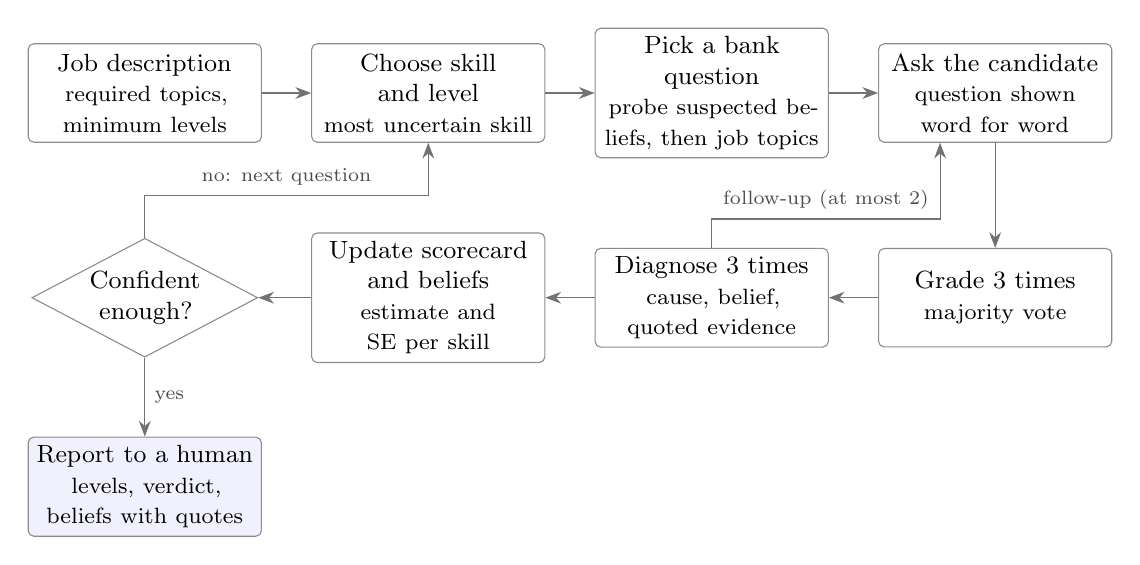
\begin{tikzpicture}[
  box/.style={draw=black!45, rounded corners=2pt, align=center, font=\small, text width=2.75cm,
              minimum height=1.25cm, inner sep=3pt},
  dec/.style={draw=black!45, diamond, aspect=1.9, align=center, font=\small, inner sep=0pt, text width=1.6cm},
  arr/.style={-{Stealth[length=2mm]}, black!55},
  lbl/.style={font=\scriptsize, text=black!70}]
  \node[box] (job)    at (0,0)     {Job description\\\footnotesize required topics, minimum levels};
  \node[box] (choose) at (3.6,0)   {Choose skill and level\\\footnotesize most uncertain skill};
  \node[box] (pick)   at (7.2,0)   {Pick a bank question\\\footnotesize probe suspected beliefs, then job topics};
  \node[box] (ask)    at (10.8,0)  {Ask the candidate\\\footnotesize question shown word for word};
  \node[box] (grade)  at (10.8,-2.6) {Grade 3 times\\\footnotesize majority vote};
  \node[box] (diag)   at (7.2,-2.6)  {Diagnose 3 times\\\footnotesize cause, belief, quoted evidence};
  \node[box] (update) at (3.6,-2.6)  {Update scorecard and beliefs\\\footnotesize estimate and SE per skill};
  \node[dec] (stop)   at (0,-2.6)    {Confident enough?};
  \node[box, fill=blue!6] (report) at (0,-5.0) {Report to a human\\\footnotesize levels, verdict, beliefs with quotes};
  \draw[arr] (job) -- (choose);
  \draw[arr] (choose) -- (pick);
  \draw[arr] (pick) -- (ask);
  \draw[arr] (ask) -- (grade);
  \draw[arr] (grade) -- (diag);
  \draw[arr] (diag) -- (update);
  \draw[arr] (update) -- (stop);
  \draw[arr] (stop) -- node[lbl, right] {yes} (report);
  \draw[arr] (stop.north) -- (0,-1.3) -- node[lbl, above, pos=0.5] {no: next question} (3.6,-1.3) -- (choose.south);
  \draw[arr] (diag.north) -- (7.2,-1.6) -- node[lbl, above, pos=0.5] {follow-up (at most 2)} (10.1,-1.6) -- (10.1,-1.6 |- ask.south);
\end{tikzpicture}
\caption{One interview of the full system (A2E). The LLM grades, diagnoses and writes follow-up
questions; code makes every decision (which question, when to stop, the verdict).}
\label{fig:loop}
\end{figure}

Figure~\ref{fig:loop} shows the loop. The LLM is used only where language is needed. Everything
that controls the interview (which question, when to stop, the verdict rule) is plain code, so the
candidate cannot change the procedure by asking.

\paragraph{Scorecard.} Each skill has an ability value $\theta$ on a logit scale. Questions come in
three levels with difficulty $b = -1, 0, +1$. An answer earns 0, 1 or 2 marks, and we model the
chance of each mark with the Partial Credit Model \cite{masters1982}:
\[
  P(X = x \mid \theta, b) \;\propto\; \exp\Big(\sum_{k \le x} (\theta - \delta_k)\Big),
  \qquad \delta_1 = b - 0.5,\; \delta_2 = b + 0.5 .
\]
We start from a normal prior (mean 0, standard deviation 1) and update it on a grid after every
graded question. The estimate is the posterior mean (EAP, \cite{bock1982}) and the uncertainty is
the posterior standard deviation (SE). Each answer is graded three times; if the marks disagree, it
counts as weaker evidence (2 of 3 agreeing gives weight 0.67). The estimate becomes a level 0--3 with
cut points at $\theta = -1.25$, $-0.25$ and $0.75$, set on stub runs in the mid-term work so that
the fixed baseline is not biased upwards.

\paragraph{Choosing the next question.} The next skill is the one with the highest SE, and the
level is the one whose difficulty is closest to that skill's estimate. Among the unasked bank
questions of that skill and level, the system prefers, in order: a question listing a misconception
it already suspects; a question on a topic the candidate just got wrong; a question on a topic the
job needs that has not been tested yet. Remaining ties are broken by a seeded random choice.

\paragraph{Stopping.} The interview stops when every skill has at least two answers and an SE
below 0.6, or after 15 main questions. We chose 0.6 for accuracy rather than length, as the
mid-term report explains.

\paragraph{Grading and follow-ups.} The grader marks the main answer three times. A follow-up is
asked when the diagnosis is not a plain knowledge gap, at most two per question. The grader then
marks the \emph{whole exchange} three times, and that final grade updates the scorecard. A reply
that shows a listed misconception scores 0 even if other parts are right.

\paragraph{Verdict.} For each skill the system computes the posterior probability that $\theta$ is
at or above the job's minimum level. Above 0.8 the skill meets the minimum, below 0.2 it does not,
otherwise it is uncertain. The verdict is \emph{not fit} if any skill is clearly below, \emph{fit} if
all clearly meet, and \emph{needs human review} otherwise.

\subsection{Tool calling}

The engine can also be run by an LLM agent instead of the code loop. The agent calls six tools
(\texttt{search\_question\_bank}, \texttt{ask\_candidate}, \texttt{grade\_answer},
\texttt{ask\_follow\_up}, \texttt{update\_scorecard}, \texttt{end\_interview}), and each tool
enforces the same rules as the code driver. A demonstration (\texttt{scripts/agent\_demo.py
--probe-rules}) runs a full interview and deliberately breaks the rules: ending before the stop rule
is met, asking a question the rules did not choose, updating the scorecard before grading, moving on
while a question is still open, and calling a tool that does not exist. All five are refused with a
reason, the agent's written summary agrees with the computed decision, and the agent reaches the same
questions, levels and verdict as the code driver. The experiments use the code driver, which gives
the same result with about 55 fewer model calls per interview.

\section{Theory of mind: modelling what the candidate believes}
\label{sec:tom}

The skill scorecard answers \emph{how much} the candidate knows. The theory-of-mind component answers
\emph{what the candidate thinks}. It does four things a human interviewer does:

\begin{enumerate}[leftmargin=*]
  \item \textbf{Attribute a belief from behaviour.} From the words of an answer, infer which belief, if
  any, the candidate holds (from the question's list of known misconceptions).
  \item \textbf{Tell a false belief from other causes.} A wrong answer can come from not knowing (a
  gap), a careless slip, misreading the question, or a false belief. Only the last is a belief about
  the subject; the others call for different follow-ups and are not reported as misconceptions.
  \item \textbf{Hold beliefs as hypotheses and test them.} An attributed belief is first only
  \emph{suspected}. The interviewer then steers the interview to test it: it prefers a later question
  that would expose the same belief, and asks follow-ups aimed at it.
  \item \textbf{Revise beliefs on evidence.} A belief is \emph{confirmed} only when the candidate shows
  it again on a different question, and \emph{disputed} (withdrawn) if the candidate says the opposite.
\end{enumerate}

\begin{figure}[h]
\centering
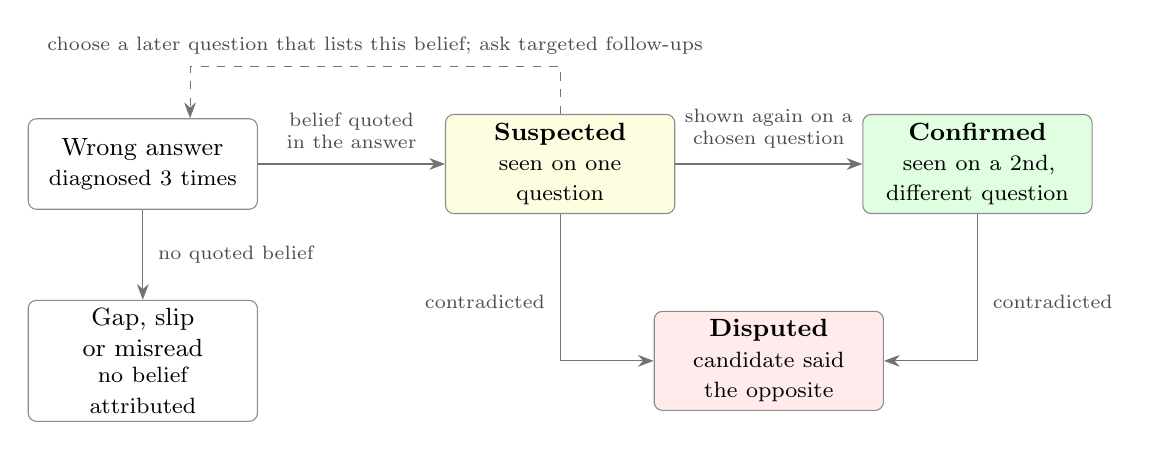
\begin{tikzpicture}[
  st/.style={draw=black!45, rounded corners=3pt, align=center, font=\small, text width=2.7cm,
             minimum height=1.15cm, inner sep=3pt},
  arr/.style={-{Stealth[length=2mm]}, black!55},
  lbl/.style={font=\scriptsize, text=black!70, align=center}]
  \node[st] (ans) at (0,0) {Wrong answer\\\footnotesize diagnosed 3 times};
  \node[st] (none) at (0,-2.5) {Gap, slip or misread\\\footnotesize no belief\\\footnotesize attributed};
  \node[st, fill=yellow!12] (sus) at (5.3,0) {\textbf{Suspected}\\\footnotesize seen on one question};
  \node[st, fill=green!12] (conf) at (10.6,0) {\textbf{Confirmed}\\\footnotesize seen on a 2nd, different question};
  \node[st, fill=red!8] (disp) at (7.95,-2.5) {\textbf{Disputed}\\\footnotesize candidate said the opposite};
  \draw[arr] (ans) -- node[lbl, above=2pt] {belief quoted\\in the answer} (sus);
  \draw[arr] (ans) -- node[lbl, right=2pt] {no quoted belief} (none);
  \draw[arr] (sus) -- node[lbl, above=2pt] {shown again on a\\chosen question} (conf);
  \draw[arr] (sus.south) |- node[lbl, pos=0.3, left=2pt] {contradicted} (disp.west);
  \draw[arr] (conf.south) |- node[lbl, pos=0.3, right=2pt] {contradicted} (disp.east);
  \draw[arr, dashed] (sus.north) -- ++(0,0.6) -| node[lbl, above=1pt, pos=0.25] {choose a later question that lists this belief; ask targeted follow-ups} ($(ans.north)+(0.6,0)$);
\end{tikzpicture}
\caption{How the system's theory of mind treats one belief. Only confirmed beliefs are reported;
disputed ones are withdrawn. Every step that needs language is done by the LLM; every state change is
made by code.}
\label{fig:tom}
\end{figure}

\paragraph{How each step is made reliable.} Figure~\ref{fig:tom} shows the life of one belief.
\begin{itemize}
  \item \textbf{Three votes with evidence.} The diagnoser runs three times. A vote that attributes a
  belief must quote the words in the candidate's answer that show it and say why. Code checks that the
  quote really is in the answer; a vote without a valid quote counts as a gap. A belief needs a strict
  majority of the three votes.
  \item \textbf{Two different questions.} A question and its own follow-up count as one piece of
  evidence, so the candidate must show the belief again on a separate question.
  \item \textbf{Correct answers are read too.} If a later answer states the opposite of a suspected or
  confirmed belief, with a quote, the belief becomes disputed and is not reported.
\end{itemize}
Nothing here is learned: it is prompts plus counting rules in code (\texttt{src/part3/diagnoser.py},
\texttt{src/engine/followups.py}, \texttt{src/shared/evidence.py}). The comparison system \textbf{A4}
has no theory of mind in this sense: it runs one diagnosis on the main answer, needs no quote, asks
generic follow-ups, never steers questions towards a belief, and reports a misconception after a
single reply. Comparing A2E with A4 answers RQ2.

\paragraph{A worked example from the final run.} Candidate CAND-003 (data engineer) was planted with
the belief that a running sum (\texttt{SUM(...) OVER (ORDER BY ...)}) shows the grand total on every row.
\begin{enumerate}[leftmargin=*]
  \item \emph{Attribution.} On question SQL-L3-010 the candidate answered: ``The query will list each
  row with the same running value equal to the total sales amount (100 + 50 + 30 + 20 = 200) for every
  day''. All three diagnosis votes attributed the belief and quoted this sentence; the belief became
  \emph{suspected}.
  \item \emph{Probing.} The follow-up asked what the running sum would show on day 2 of a three-day
  table; the candidate replied ``It would show the overall total''. This is more evidence from the
  same question, so the belief stayed suspected.
  \item \emph{Testing on a new question.} Six questions later the system chose SQL-L3-012 with the
  recorded reason ``lists a suspected misconception to confirm''. The candidate wrote: ``Adding
  \texttt{ORDER BY order\_date} inside the OVER clause just sorts the rows, so every row still shows the
  overall total for that customer.'' The belief was \emph{confirmed}, with both quotes in the report.
\end{enumerate}
The same candidate's report also listed two beliefs as only suspected, so a human reading it can see
which attributions are firm and which are hypotheses.

\paragraph{Revising a belief.} For CAND-006 the system first attributed the belief that Python's
\texttt{or} evaluates both sides, from ``the right side is still evaluated''. In the follow-up the
candidate said the opposite: ``Because the overall result is already determined to be true, the right
side is never executed or needed.'' The belief was marked disputed and not reported, which was
correct: it was not one of the candidate's planted beliefs. Without this revision, the report would
have accused the candidate of a misconception they do not hold.

\paragraph{A correction before the final run.} The quote check first required an exact character
match. In the first final-run attempt we found that the candidate model writes narrow no-break
spaces and backticks around code, which Gemini drops when it quotes, so correct diagnoses with
correct quotes were being discarded. In a replay of that attempt's diagnoses, 32 of the 150
misconception votes (21\%) were rejected for formatting alone. We changed the check to ignore spaces,
backticks, quotation marks and letter case; the quote must still be the candidate's own words, and
the stored evidence is the exact span of the answer. The attempt was discarded and the final run
restarted under a new version with this fix (Section~\ref{sec:setup}).


\section{Data}

\paragraph{Question bank.} 135 questions: 3 skills $\times$ 3 levels $\times$ 15, each with a model
answer, key points, a 0/1/2 rubric, topic tags and a list of common misconceptions. There are
\emph{explain} and \emph{read-code} questions. Questions were drafted with an LLM; every question was
then reviewed by a teammate for answer correctness, rubric consistency, relevant misconceptions and
level. The review flagged 66 questions and we corrected 43 (wrong claims in model answers, unclear
wording, and misconceptions listed on questions that do not test them). The other notes asked for
rubric changes our grading rule already covers. Level notes were resolved by aligning the written
level definitions with the topic levels the bank was built from, without moving questions.

\paragraph{Misconceptions.} 95 misconceptions. Where a published catalogue exists we adapted from
it: Progmiscon for Python \cite{chiodini2021}, a think-aloud study of SQL novices
\cite{miedema2021}, concept-inventory work on data structures \cite{karpierz2014} and the McMining
benchmark \cite{alhossami2025}. The rest were written for this project.

\paragraph{Jobs.} Three job descriptions (junior data analyst, backend engineer, data engineer),
each with a minimum level per skill and 13 to 17 required topics.

\paragraph{Simulated candidates.} Each candidate has a hidden answer key: a level (0--3) for every
topic, one or two planted misconceptions, and small chances of misreading or slipping. A
candidate's true level for a skill is the floor of their mean level over the topics the job
requires; planted misconceptions do not change it. Candidates come in blocks of 12 that cover every
combination of job, even or uneven profile, and fit or not fit once. For every question, code decides
what the candidate should do (answer correctly, partly, wrongly, with a planted misconception,
misread, or slip) and a second LLM writes the answer following that plan.

\section{Experimental setup}
\label{sec:setup}

\begin{table}[h]
\centering\small
\begin{tabularx}{\linewidth}{@{}l X l@{}}
\toprule
System & What it is & Compared with \\
\midrule
B1 & Fixed: 12 questions (levels 1, 2, 2, 3 per skill), no follow-ups, no diagnosis & -- \\
ADAPT12 & Adaptive question choice, exactly 12 questions, no follow-ups, no diagnosis & B1 (RQ1, equal length) \\
A2E & Full system: adaptive choice, early stopping, theory of mind of the candidate & B1 (RQ1), A4 (RQ2) \\
A4 & A2E without the theory of mind (single diagnosis, no quotes, no belief testing, one-reply confirmation) & A2E (RQ2) \\
A5E & A2E with job-blind question choice & A2E (job-aware retrieval) \\
\bottomrule
\end{tabularx}
\caption{The five systems. Every system interviewed every candidate.}
\label{tab:systems}
\end{table}

\paragraph{Models.} Grading, diagnosis and topic extraction use \texttt{gemini-3.5-flash-lite}; the
simulated candidate is \texttt{gpt-oss-120b} on Groq, a different model family. Before the run, one
interview each of B1 and A2E on a separate validation candidate checked that every grade and
diagnosis got three valid votes.

\paragraph{Runs.} Candidates were run one at a time through all five systems, in the order of the
balanced blocks, so that every finished candidate has a result from every system. The run covers
\fN{} complete candidates (\fInterviews{} interviews). The first block of 12 is complete and
balanced; the second is missing two candidates. Every comparison below uses the
same \fN{} candidates in every system. The run's manifest fingerprints the source code, bank, prompts,
models and candidate files, and results from a different setup cannot be mixed in.

\paragraph{Metrics.} \emph{Skill accuracy} is the share of (candidate, skill) pairs where the
reported level equals the true level; we also report the mean absolute level error.
\emph{Exchanges} are main questions plus follow-ups. \emph{Verdicts} are right, wrong, or sent to a
human. \emph{Misconception recall} is the share of planted misconceptions that were confirmed, and
\emph{precision} the share of confirmed misconceptions that were planted. The \emph{false-alarm rate}
is the share of replies planned as correct on which a misconception was named.

\paragraph{Uncertainty.} With \fN{} candidates the numbers move a lot from sample to sample, so we
give 95\% bootstrap intervals: candidates are redrawn with replacement 2,000 times, with the same
draw for every system because they interviewed the same people. For a comparison the interval is
for the difference between the two systems.

\section{Results}
\label{sec:results}

\begin{table}[h]
\centering\small
\begin{tabular}{@{}lccccc@{}}
\toprule
 & B1 & ADAPT12 & A2E & A5E & A4 \\
\midrule
Skill levels right & \fAccBOne{} & \fAccAdapt{} & \fAccFull{} & \fAccBlind{} & \fAccAfour{} \\
Mean level error & \fMaeBOne{} & \fMaeAdapt{} & \fMaeFull{} & \fMaeBlind{} & \fMaeAfour{} \\
Exchanges per interview & \fExchBOne{} & \fExchAdapt{} & \fExchFull{} & \fExchBlind{} & \fExchAfour{} \\
Verdicts right / to a human / wrong & \fRightBOne{} / \fReviewNBOne{} / \fWrongBOne{} & \fRightAdapt{} / \fReviewNAdapt{} / \fWrongAdapt{}
  & \fRightFull{} / \fReviewNFull{} / \fWrongFull{} & \fRightBlind{} / \fReviewNBlind{} / \fWrongBlind{} & \fRightAfour{} / \fReviewNAfour{} / \fWrongAfour{} \\
Misconception recall & -- & -- & \fRecallFull{} & \fRecallBlind{} & \fRecallAfour{} \\
Misconception precision & -- & -- & \fPrecisionFull{} & \fPrecisionBlind{} & \fPrecisionAfour{} \\
False alarms on correct replies & -- & -- & \fFalseAlarmFull{} & \fFalseAlarmBlind{} & \fFalseAlarmAfour{} \\
Required job topics tested & \fCoverageBOne{} & \fCoverageAdapt{} & \fCoverageFull{} & \fCoverageBlind{} & \fCoverageAfour{} \\
Interviewer LLM calls & \fCallsBOne{} & \fCallsAdapt{} & \fCallsFull{} & \fCallsBlind{} & \fCallsAfour{} \\
\bottomrule
\end{tabular}
\caption{All five systems on the same \fN{} candidates (\fPlanted{} planted misconceptions).}
\label{tab:main}
\end{table}

\subsection{RQ1: skill levels and length}

\begin{figure}[h]
\centering
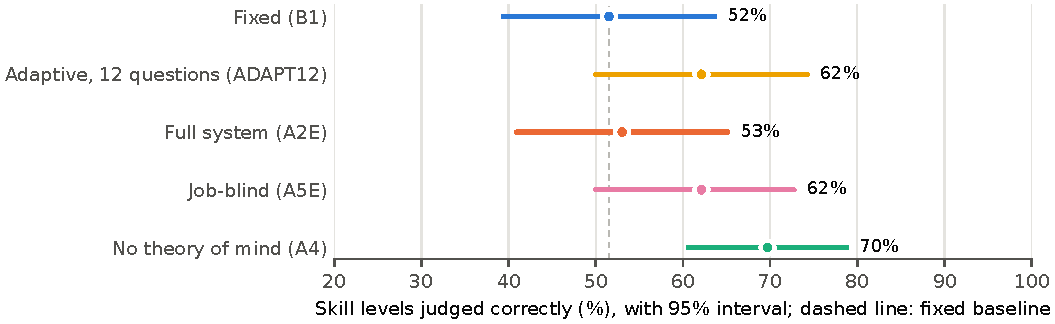
\includegraphics[width=0.88\linewidth]{final_accuracy}
\caption{Skill levels judged correctly, with 95\% intervals over candidates.}
\label{fig:accuracy}
\end{figure}

\paragraph{Adaptive choice at equal length.} ADAPT12 and B1 both ask exactly 12 questions; only the
choice of questions differs. ADAPT12 judged \fAccAdapt{} of levels correctly against \fAccBOne{}, a
difference of \fAdaptVsFixedSkillAccuracyDiff{} points \ci{\fAdaptVsFixedSkillAccuracyLow}{\fAdaptVsFixedSkillAccuracyHigh}.
The interval includes a small loss, so we read this as a likely gain from adaptivity rather than a
proven one. It repeats the direction of the mid-term stub controls, now with the live models.

\paragraph{The full system against the fixed interview.} A2E judged \fAccFull{} of levels
correctly, a difference of \fFullVsFixedSkillAccuracyDiff{} points from B1
\ci{\fFullVsFixedSkillAccuracyLow}{\fFullVsFixedSkillAccuracyHigh}: no measurable gain. It asked
\fExchFull{} exchanges per interview against \fExchBOne{} (difference \fFullVsFixedMeanExchangesDiff{}
\ci{\fFullVsFixedMeanExchangesLow}{\fFullVsFixedMeanExchangesHigh}), mostly follow-ups
(Figure~\ref{fig:length}). RQ1's target of 25\% fewer exchanges is not met. Its errors are not one
sided: \fOverFull{} levels too high and \fUnderFull{} too low, where B1 errs mostly upwards
(\fOverBOne{} and \fUnderBOne{}).

\begin{figure}[h]
\centering
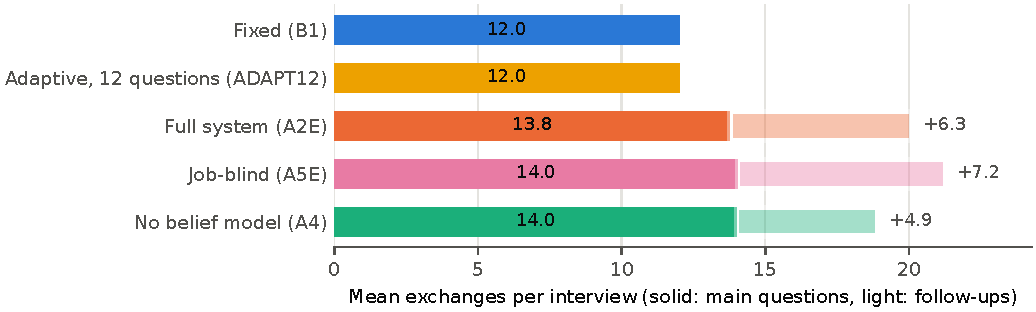
\includegraphics[width=0.88\linewidth]{final_length}
\caption{Interview length: main questions plus follow-ups.}
\label{fig:length}
\end{figure}

\paragraph{Verdicts.} No adaptive system passed an unfit candidate or rejected a fit one; B1 passed
one unfit candidate (Figure~\ref{fig:verdicts}). All systems send many candidates to a
human (between a third and 60\%), because the 0.8 rule demands a clear margin above the job minimum. A4 decided the most cases
(\fRightAfour{} of \fN{}), in line with its better level estimates.

\begin{figure}[h]
\centering
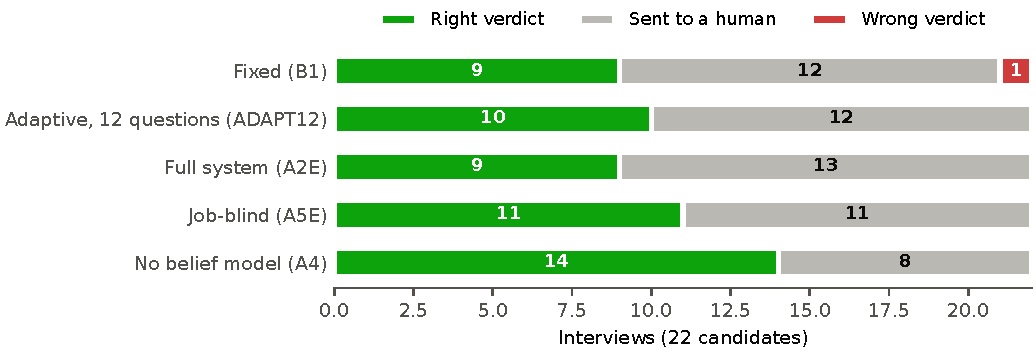
\includegraphics[width=0.88\linewidth]{final_verdicts}
\caption{Fit / not-fit verdicts per system.}
\label{fig:verdicts}
\end{figure}

\subsection{RQ2: does the theory of mind help?}

\begin{figure}[h]
\centering
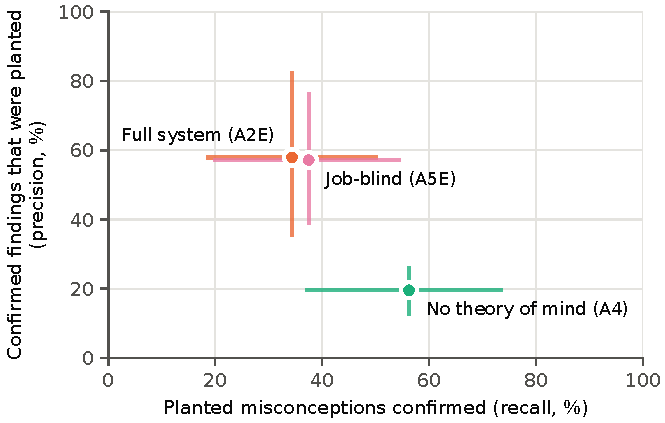
\includegraphics[width=0.62\linewidth]{final_beliefs}
\caption{Recall against precision of confirmed misconceptions, with 95\% intervals. Up is more
trustworthy, right finds more.}
\label{fig:beliefs}
\end{figure}

Figure~\ref{fig:beliefs} shows the trade-off. Without the theory of mind, A4 confirmed
\fConfirmedAfour{} misconceptions in \fN{} interviews and found \fFoundAfour{} of the \fPlanted{}
planted ones (recall \fRecallAfour{}), but only \fPrecisionAfour{} of its findings were planted. With
the theory of mind, A2E confirmed \fConfirmedFull{} and found \fFoundFull{} (recall \fRecallFull{}),
and \fPrecisionFull{} of its findings were planted:

\begin{center}\small
\begin{tabular}{@{}lccc@{}}
\toprule
A2E $-$ A4 & Difference & 95\% interval \\
\midrule
Precision & \fFullVsAfourPrecisionDiff{} points & \fFullVsAfourPrecisionLow{} to \fFullVsAfourPrecisionHigh{} \\
Recall & \fFullVsAfourRecallDiff{} points & \fFullVsAfourRecallLow{} to \fFullVsAfourRecallHigh{} \\
False alarms on correct replies & \fFullVsAfourFalseAlarmRateDiff{} points & \fFullVsAfourFalseAlarmRateLow{} to \fFullVsAfourFalseAlarmRateHigh{} \\
\bottomrule
\end{tabular}
\end{center}

\noindent Both differences are clear. For a screening tool, precision matters more: telling a
candidate they hold a misconception they do not is worse than missing one, and A4 is wrong about four
times in five. The theory of mind also kept \fSuspectedFull{} beliefs as hypotheses only (seen on one
question) and withdrew \fDisputedFull{} after the candidate contradicted them, none of them planted;
neither counts as a finding, but both are visible to the human reading the report. Neither system named a misconception on a correctly answered reply. The recall target of
60\% from the proposal is not met. Precision here is against planted misconceptions only: a
simulated candidate told to answer wrongly sometimes states a common misconception that was not
planted, so some ``false'' findings may be right about the reply.

\subsection{Why the full system is less accurate on levels than A4}
\label{sec:levels-why}

A4 judged \fAccAfour{} of levels correctly and A2E \fAccFull{}, a difference of
\fFullVsAfourSkillAccuracyDiff{} points \ci{\fFullVsAfourSkillAccuracyLow}{\fFullVsAfourSkillAccuracyHigh}.
Both use the same scorecard, question-choice rules and stopping rule, so the difference comes
from the theory of mind. To confirm a belief on a second question, A2E prefers questions that list a suspected
misconception. A candidate who holds it answers those wrongly by design. A2E asked \fHeldBeliefFull{}
such questions per interview, A4 \fHeldBeliefAfour{} and B1 \fHeldBeliefBOne{}. Each scores 0 and
pulls the estimate down, but the true level ignores planted misconceptions, so the result shows up
as under-estimates: \fUnderFull{} of A2E's wrong levels are too low, against \fUnderAfour{} for A4.
This is a real cost of probing beliefs, partly made larger by our definition of the true level. A
system that wants both could keep the probing questions out of the level estimate, or stop probing
once a belief is confirmed.

\subsection{Premature stops}

An interview stops early when every skill's SE is below 0.6. A2E stopped this way in
\fConfStopsFull{} of \fN{} interviews, and after those stops \fConfWrongFull{} of \fConfSkillsFull{}
skill levels were wrong (A4: \fConfWrongAfour{} of \fConfSkillsAfour{}).
\begin{itemize}
  \item \textbf{By skill:} Python \fConfWrongPyFull{}, data structures \fConfWrongDsFull{}, SQL
  \fConfWrongSqlFull{} wrong levels out of 20 each. SQL is judged best.
  \item \textbf{By size:} all but \fConfTwoOffFull{} of the wrong levels after an early stop are one
  level off; the rule stops as soon as the estimate is precise enough, even when it sits next to a cut
  point.
  \item \textbf{At the bottom of the scale:} \fZeroWrongFull{} of the \fZeroFull{} skills a candidate
  did not know at all (true level 0) were reported as level 1.
\end{itemize}
SE below 0.6 means the estimate is precise, not that it is far from a cut point. Asking one more
question when the estimate is close to a cut point, or requiring most of the posterior to lie in one
level, would address this; the second rule was implemented (A2EB) but not run live.

\subsection{Job-aware question choice}

A5E differs from A2E only in ignoring the job description when choosing questions. It tested fewer
of the job's required topics (\fCoverageBlind{} against \fCoverageFull{}, a difference of
\fBlindVsFullTopicCoverageDiff{} points \ci{\fBlindVsFullTopicCoverageLow}{\fBlindVsFullTopicCoverageHigh}),
which is what job-aware retrieval is for. Its level accuracy and misconception recall were not
measurably different (\fBlindVsFullSkillAccuracyDiff{} points
\ci{\fBlindVsFullSkillAccuracyLow}{\fBlindVsFullSkillAccuracyHigh} on levels). So job-aware choice
makes the interview cover the job, without a measurable effect on accuracy at this sample size.

\subsection{Cost}

A2E made \fCallsFull{} interviewer-side LLM calls per interview against \fCallsBOne{} for B1: three
grading and three diagnosis votes per answer, including correct ones. A4 needed \fCallsAfour{}.

\section{Discussion}

\begin{table}[h]
\centering\small
\begin{tabularx}{\linewidth}{@{}lXll@{}}
\toprule
& Target & Result & Status \\
\midrule
RQ1 & Skill accuracy within 5 points of B1 & \fFullVsFixedSkillAccuracyDiff{} points \ci{\fFullVsFixedSkillAccuracyLow}{\fFullVsFixedSkillAccuracyHigh} & \open \\
RQ1 & At least 25\% fewer exchanges than B1 & \fExchFull{} against \fExchBOne{} & \fail \\
RQ1 & Adaptive choice beats the fixed list at equal length & \fAdaptVsFixedSkillAccuracyDiff{} points \ci{\fAdaptVsFixedSkillAccuracyLow}{\fAdaptVsFixedSkillAccuracyHigh} & \open \\
RQ2 & More trustworthy belief attributions than without the theory of mind & \fFullVsAfourPrecisionDiff{} points precision & \pass \\
RQ2 & Misconception recall of at least 60\% & \fRecallFull{} & \fail \\
RQ2 & False alarms on correct answers below 15\% & \fFalseAlarmFull{} & \pass \\
\bottomrule
\end{tabularx}
\caption{The targets against the final results.}
\label{tab:targets}
\end{table}

\paragraph{What we learned.} The theory of mind works where it matters most for a screening tool:
when it says a candidate holds a misconception, it is right most of the time, it never says so about
a correct answer, and it withdraws a belief when the candidate contradicts it. A system without it
finds more planted beliefs only by attributing beliefs freely, and four in five of its attributions
are wrong. The mid-term version, whose confirmations could come from a single question, had the same
problem (18\% precision); testing each belief on a second question and requiring the candidate's own
words fixed it. Adaptive question choice also does what adaptive testing promises: at the same length
it places candidates better than a fixed list, though our sample cannot prove it. The two do not
combine for free. Confirming a belief needs evidence from a second question,
and that evidence comes from deliberately probing a weakness, which costs level accuracy and length.
A2E is therefore not the best system on every measure: A4 judges levels best and ADAPT12 is the
best short interview, but only A2E gives a trustworthy account of \emph{what the candidate believes}
and why they are wrong.

\paragraph{Mid-term against final.} In the mid-term, A2 beat B1 on levels by 17 points. With A2E on
the reviewed bank and new candidates it does not. Two things changed: the stricter belief
model (which probes more, as shown above) and the corrected question bank; the candidates are the
same people (the first 22 of the 24 used then). The mid-term gain also included more
questions, as that report noted, and our final equal-length comparison is the cleaner test of
adaptivity.

\paragraph{The evidence check matters.} A rule that checks the model's evidence is only as good as the
check. An exact-match rule silently threw away a fifth of correct diagnoses because of invisible
formatting differences between two models. Checking evidence against real outputs, not only test
cases, caught it.

\section{Limitations}

\begin{itemize}
  \item \textbf{Simulated candidates.} Real candidates are less consistent. The simulated candidate
  sometimes ignored its plan (graded answers matched the plan for \fGradingMatchFull{} of A2E's
  questions), and a follow-up occasionally gave the answer away, after which the grader gave full
  marks. Results describe the interviewer against a controlled population.
  \item \textbf{Sample size.} \fN{} candidates give wide intervals; several comparisons are not
  settled. Running all 60 candidates would narrow them.
  \item \textbf{Truth ignores misconceptions.} A candidate's true level does not count planted
  misconceptions, which favours systems that do not probe them (Section~\ref{sec:levels-why}).
  \item \textbf{One grader model, no human check yet.} Every grade comes from one Gemini model. The
  planned hand checks were not done: two teammates independently marking a sample of answers against
  the rubric, and labelling 30 simulated answers against their plans, reporting Cohen's $\kappa$
  between them with $\kappa \ge 0.6$ as acceptable. If $\kappa$ is lower, the labelling guide is
  ambiguous: we would rewrite it, settle the disagreements together and label a fresh sample. If the
  two agree with each other but not with the model, the fault is the model's: we would report the
  grader's error rate beside every accuracy figure, and score simulated answers against what was
  written rather than the plan.
  \item \textbf{Settings tuned before A2E.} The stopping threshold and cut points were tuned on stub
  runs before the theory-of-mind component was changed.
  \item \textbf{Safety.} Only one manipulation attempt per system was in this sample. It did not raise
  the grade and was flagged, but one case shows little.
\end{itemize}

\section{Conclusion and future work}

We built an interviewer with an explicit theory of mind of the candidate: it attributes beliefs from
what the candidate says, tells a false belief from a gap, a slip or a misreading, holds each belief as
a hypothesis, steers the interview to test it, and confirms or withdraws it on evidence in the
candidate's own words. Alongside, it estimates skill levels adaptively and leaves the hiring decision
to a human. On \fN{} simulated candidates, the theory of mind made belief attributions about three
times as trustworthy as a version without it (\fPrecisionFull{} against \fPrecisionAfour{}), and
adaptive question choice placed candidates better than a fixed list at equal length. The full system
did not combine both advantages: testing beliefs cost level accuracy and length. The most useful next steps are to keep
belief-probing questions out of the level estimate, to stop probing a belief once it is confirmed, to
require a clear margin from the nearest cut point before stopping, to finish the run on all 60
candidates, and to complete the human checks.

\section*{Reproducing this report}
\begingroup\sloppy
Code, question bank and candidates are at \url{https://github.com/Srinjoy003/LMA-RAG}. The final
run is \texttt{reviewed-main-v2}, produced by \texttt{scripts/run\_rotating.py} in the order of
\texttt{docs/final\_run\_order.txt}; its manifest records the code, bank, prompts and models. Every
result number and figure in this report is generated by \texttt{report/make\_final\_figures.py}
from the \fN{} complete candidates, and \texttt{scripts/evaluate.py} gives the full metric table.
Every LLM response is cached on disk, so re-running from the cache gives the same interviews.
\par\endgroup

\begin{thebibliography}{99}\small
\bibitem{alhossami2025} E.~Al-Hossami and R.~Bunescu. McMining: automated discovery of
  misconceptions in student code. In \emph{EACL} (short papers), 2026. arXiv:2510.08827.
\bibitem{bock1982} R.~D.~Bock and R.~J.~Mislevy. Adaptive EAP estimation of ability in a
  microcomputer environment. \emph{Applied Psychological Measurement}, 6(4):431--444, 1982.
\bibitem{chiodini2021} L.~Chiodini, I.~Moreno Santos, A.~Gallidabino, A.~Tafliovich, A.~L.~Santos
  and M.~Hauswirth. A curated inventory of programming language misconceptions. In \emph{ITiCSE},
  pages 380--386, 2021.
\bibitem{karpierz2014} K.~Karpierz and S.~A.~Wolfman. Misconceptions and concept inventory
  questions for binary search trees and hash tables. In \emph{SIGCSE}, pages 109--114, 2014.
\bibitem{masters1982} G.~N.~Masters. A Rasch model for partial credit scoring.
  \emph{Psychometrika}, 47(2):149--174, 1982.
\bibitem{miedema2021} D.~Miedema, E.~Aivaloglou and G.~Fletcher. Identifying SQL misconceptions of
  novices: findings from a think-aloud study. In \emph{ICER}, pages 355--367, 2021.
\bibitem{yu2025} J.~Yu, Y.~Zhuang, Y.~Sun, W.~Gao, Q.~Liu, M.~Cheng, Z.~Huang and E.~Chen.
  TestAgent: an adaptive and intelligent expert for human assessment. In \emph{Findings of ACL},
  pages 724--747, 2025.
\bibitem{zhuang2024} Y.~Zhuang, Q.~Liu et al. Survey of computerized adaptive testing: a machine
  learning perspective. arXiv:2404.00712, 2024. Accepted to \emph{IEEE TPAMI}.
\end{thebibliography}

\end{document}
